\chapter{Funkční testy}
\label{testovani}
\section{Napájení}
Na základní desce jsou generované celkem 3 napájecí úrovně z +5 V externího napájení USB, jak bylo uvedeno v sekci \ref{napajeni}. A to napájecí úrovně +1.2 V, +2.5 V a +3.3 V. Parametry generovaných napájení budou uvedeny v následujících částech.

%TODO jak uvest zatez?
\subsection{Zvlnění výstupních napětí}
 Zvlnění výstupních napětí bylo vždy měřeno co nejblíže výstupu každého spínaného regulátoru se snahou vytvoření co nejkratší zemní smyčky mezi měřícím bodem a připojenou zemnící sondou osciloskopu. Měření nebylo ve všech případech s ohledem na velikost zemní smyčky ideální vzhledem k zapojení ve kterém je realizováno vyčítací rozhraní a to tedy v zapojení, kdy je deska s Timepix 2 nad základní deskou a tedy není možné se připojit sondou osciloskopu na vrchní stranu základní desky, která se nachází pod deskou s detektorem Timepix 2. I s ohledem na zmíněné problémy byly naměřeny tyto průběhy \ref{fig:napeti} zvlnění výstupních napětí. Kde CH3: +2.5 V, CH2: +3.3V a CH1: +1.2 V.  
\begin{figure}[h!]
	\centering
	\captionsetup{justification=centering}
	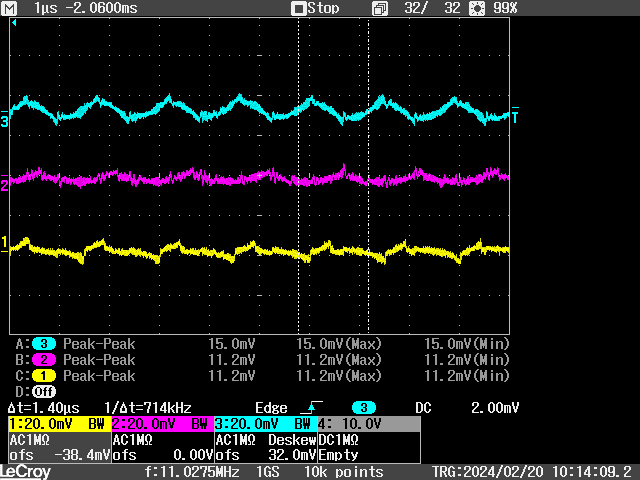
\includegraphics[scale=0.40]{./Mereni/ripple 3V3 - CH2 & 2V5 - CH3 & 1V2 - CH1, 2x 47uF.png}
	\caption{Zvlnění výstupních napětí +2.5V, +3.3 V a +1.2 V, generovaných na základní desce \ref{zakladni deska}.} 
	\label{fig:napeti}
\end{figure}
Výsledné hodnoty zvlnění výstupních napětí je možné najít v uvedené tabulce \ref{tab:zvlneni}.
\begin{table}[h!]
	\centering
	\begin{tabular}{ |P{2cm}|P{4cm}|P{4cm}|P{3cm}|  }
		\hline
		\multicolumn{4}{|c|}{Parametry výstupních napětí} \\
		\hline
		Typ napětí & Max. Zvlnění [mV] & RMS max. [V] & RMS min. [V]\\ \hline \hline 
		+1.2 V & 11.2 & 1.22 & 1.21\\ \hline 	
		+2.5 V & 15.0 & 2.57 & 2.55\\ \hline
		+3.3 V & 11.2 & 3.30 & 3.28\\ \hline
	\end{tabular}
	\caption{Parametry výstupních napětí}
	\label{tab:zvlneni}
\end{table}

\subsection{Stejnosměrné úrovně výstupních napětí}
Stejnosměrné hodnoty výše uvedených napájecích úrovní je možné vidět na obrázku \ref{fig:urovne}. Shrnující údaje o stejnosměrné hodnotě výstupního napětí lze také dohledat z tabulce \ref{tab:zvlneni}.
\begin{figure}[h!]
	\centering
	\captionsetup{justification=centering}
	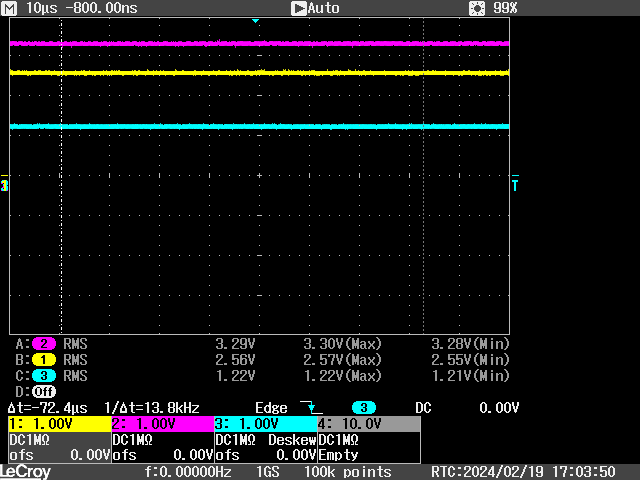
\includegraphics[scale=0.40]{./Mereni/vout 3V3 & 2V5 & 1V2.png}
	\caption{Stejnosměrné úrovně výstupních napětí, +2.5V, +3.3 V a +1.2 V, spínaných regulátorů na základní desce \ref{zakladni deska}.} 
	\label{fig:urovne}
\end{figure}

\subsection{Napájecí sekvence}
Ověření rozfázování napájecí sekvence je uvedeno na obrázku \ref{fig:napajeci_sekvecne_real}. Kde CH1 je napájení +1.2 V, CH2 je +2.5 V a CH3 je vstupních +5V. Při tomto měření byl vstupní pin EN regulátoru pro +2.5 V propojen s výstupním pinem PG, regulátoru s výstupním napětím +3.3 V. Na nastavených kurzorech je také vidět, že teoreticky vypočítaný čas \ref{eq:Tss}, doby rozběhu regulátoru z rovnice \ref{eq:Tss}, souhlasí s prakticky naměřenými hodnoty. 
\begin{figure}[h!]
	\centering
	\captionsetup{justification=centering}
	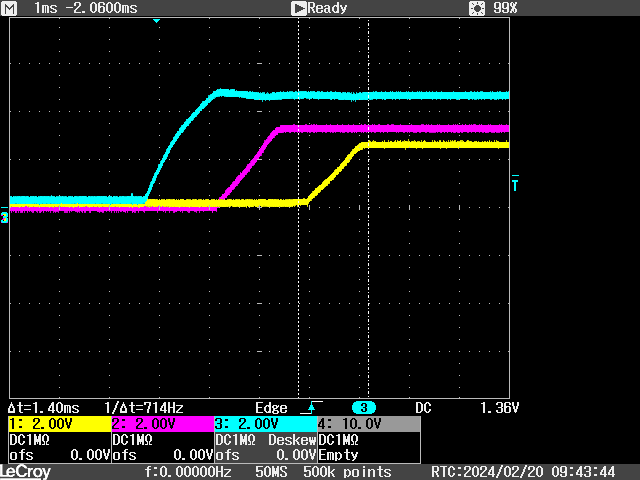
\includegraphics[scale=0.45]{napajeci_sekvence_real.png}
	\caption{Měření napájecí sekvence základní desky.} 
	\label{fig:napajeci_sekvecne_real}
\end{figure}

\subsection{Měření spotřeby}
%TODO zmenit nastaveni MachXO2 -: zlepsi se to ?
Měření spotřeby probíhalo měřením úbytku napětí na 100 $m\Omega$ odporu zapojeného do série v +5 V napájecí větvi. Naměřené parametry můžete vidět v tabulce \ref{tab:spotreba}. 
\begin{table}[h!]
	\centering
	\begin{tabular}{ |P{8cm}|P{2cm}|P{2cm}|  }
		\hline
		\multicolumn{3}{|c|}{Spotřeba navrženého rozhraní} \\
		\hline
		Část rozhraní & Naměřené napětí [mV] & Spotřeba [mW]\\ \hline \hline 
		Základní Deska & 8.9 & 445\\ \hline 	
		Celé rozhraní, před int. TPX2 & 16 & 800\\ \hline
		Celé rozhraní, po int. TPX2 & 29.1 & 1455\\ \hline
		Celé rozhraní, 1/2 TPX2 zamaskovaná & 21.8 & 1090\\ \hline
		Celé rozhraní, TPX2 zamaskovaný & 16.5 & 825\\ \hline
	\end{tabular}
	\caption{Spotřeba navrženého vyčítacího rozhraní}
	\label{tab:spotreba}
\end{table}

\section{Odvod tepla z vyčítacího rozhraní}
Analýzu odvodu tepla ze zařízení je možné vidět na obrázku \ref{fig:teplo}, kdy snímek byl pořízen termokamerou ve stavu, kdy navržené vyčítací rozhraní bylo v procesu ekvalizace.
\begin{figure}[h!]
	\centering
	\captionsetup{justification=centering}
	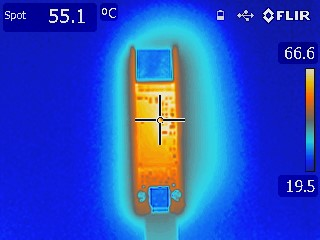
\includegraphics[scale=0.99]{./Mechanika/teplo_1.jpg}
	\caption{Odvod tepla z navrženého vyčítacího rozhraní.} 
	\label{fig:teplo}
\end{figure}

\section{USB komunikace}
Fyzická implementace USB byla popsána v části textu \ref{USB}. Pro testování USB komunikace byly použity dvě USB třídy. První třídou USB byl virtuální sériový port přes USB. Tato třída sloužila pouze pro rychlé ověření funkčnosti USB periférie. Druhou třídou byla třída RNDIS, neboli virtuální ethernet přes USB, tato třída byla použita pro přenos UDP protokolu přes USB, tedy z navrženého vyčítacího rozhraní do rozhraní uživatelského.
\subsection{Virtuální ethernet přes USB}
Hlavní USB třída, která byla použita v konečné implementaci byla třída RNDIS. Jedná se o třídu USB kdy je přes USB implementován virtuální ethernet. V této práci se konkrétně pomocí USB přenáší UDP protokol. Tato třída byla zvolena s ohledem na existující program TrackLab \cite{Manek_2024} a již existující komunikační protokol, využívající UDP komunikaci. TrackLab umožňuje připojit různá vyčítací rozhraní s pixelovými detektory. Vyčítací rozhraní v této práci respektuje již existující standart a to standart připojení vyčítacího rozhraní Katherine pro Timepix 2 \ref{Katherine}. Navržené miniaturizované rozhraní se tedy programu TrackLab jeví jako právě zmíněné, vyčítací rozhraní Katherine pro Timepix 2. Připojené vyčítací rozhraní do programu TrackLab s nastaveno ip adresou je možné vidět na obrázku \ref{fig:ip}.

\section{Vysokonapěťový zdroj}
% Nastaveni VN zdroje
Zapojení vysokonapěťového zdroje a princip měření vysokého napětí, které je generováno na desce s Timepix 2 \ref{Deska s Timepix2} je popsán v části textu \ref{VN zdroj}. Závislost zapsané 8-bitové hodnoty na výstupním napětí vysokonapěťového zdroje je možné vidět na obrázku \ref{fig:hv_hex}, kdy nastavené vysoké napětí bylo zpětnovazebně měřeno mikrokontrolérem. Nastavené vysoké napětí je poté monitorováno programem TrackLab, jak lze vidět na obrázku \ref{fig:Tracklab}.
\begin{figure}[h!]
	\centering
	\captionsetup{justification=centering}
	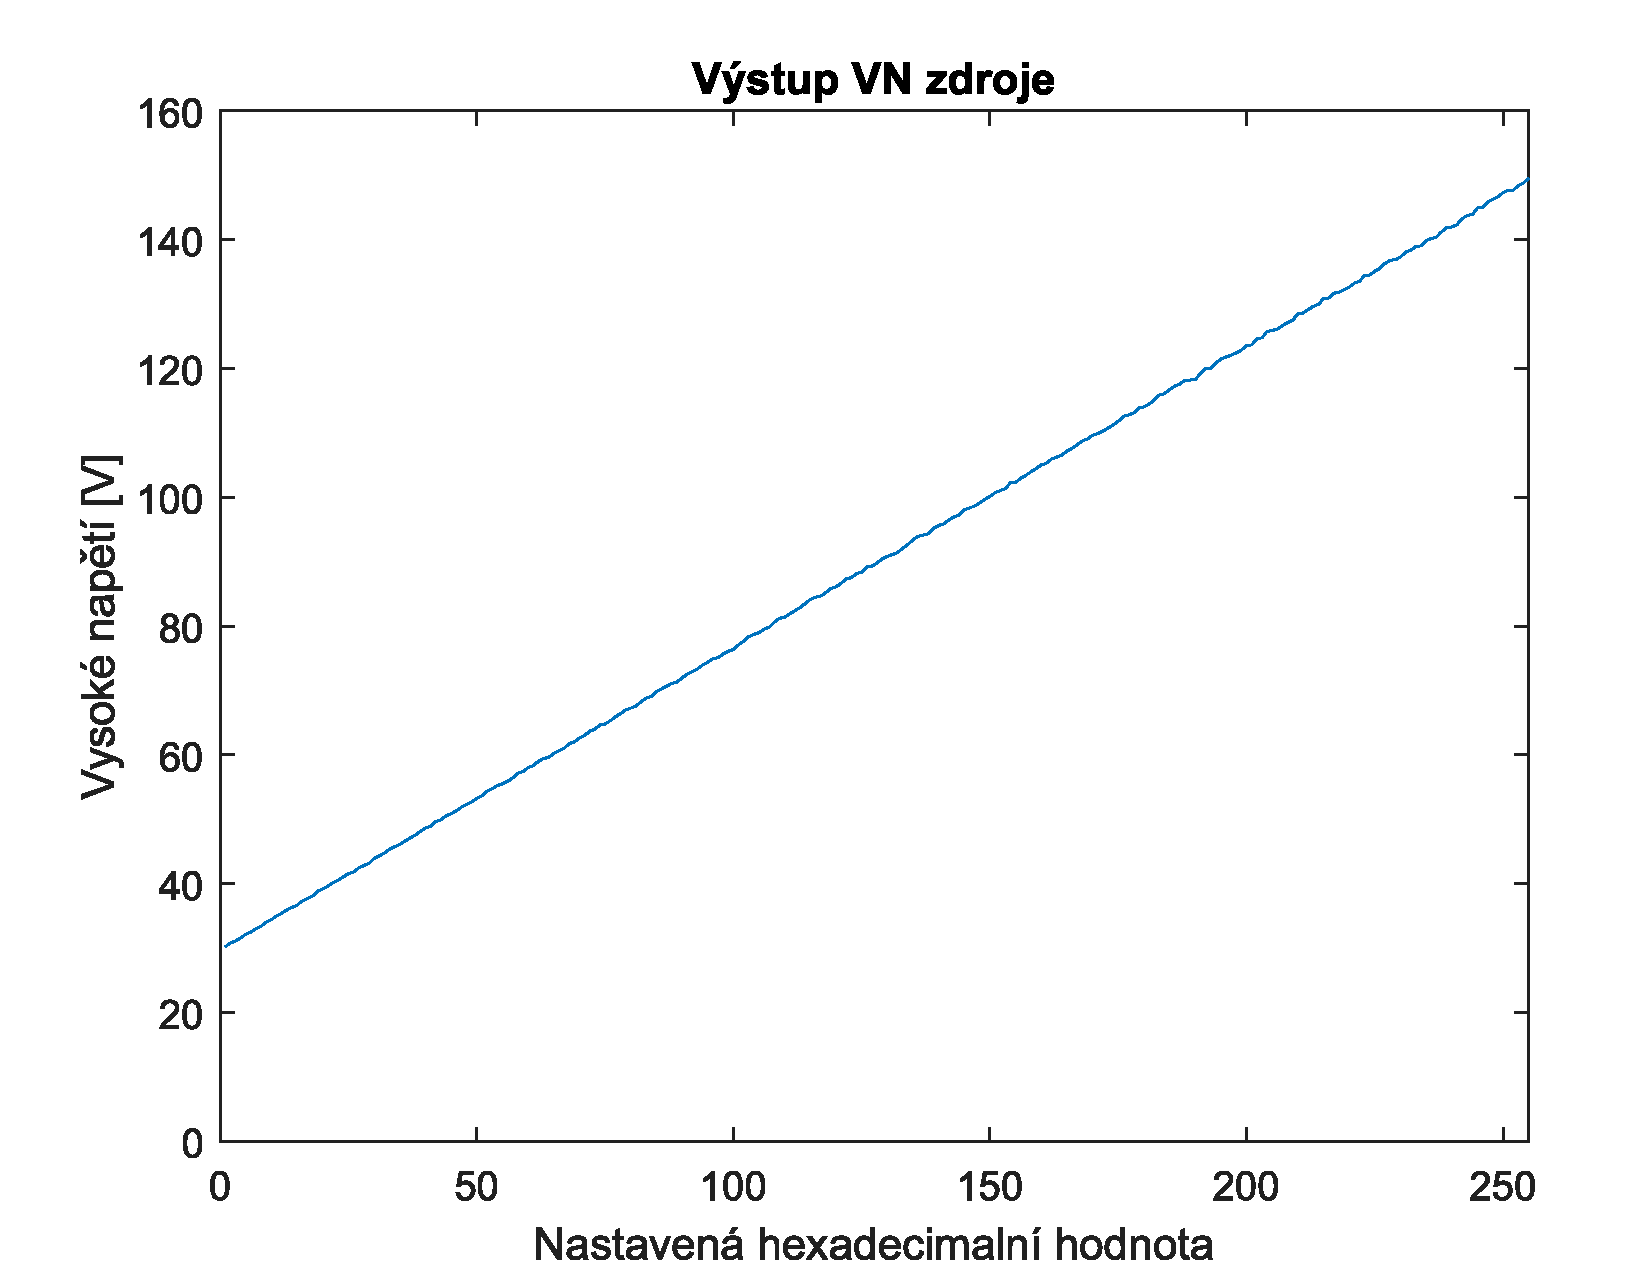
\includegraphics[scale=0.40]{./Mereni/hv_hex_small.pdf}
	\caption{Závislost vstupní 8 bitové hodnoty na výstupním napětí VN zdroje.} 
	\label{fig:hv_hex}
\end{figure}


% TODO promereni teploty s mechanikou ??, termokamra ??
\section{Měření teploty}
V této práci bylo implementováno měření teploty pomocí externího teplotního senzoru na desce s detektorem Timepix 2 \ref{Deska s Timepix2} a měření teploty za využití interního měření teploty detektoru Timepix 2. Měření teploty za využití detektoru Timepix 2, bude uvedeno v části \ref{teplota}.
\subsection{Měření teploty vyčítacího rozhraní}
Typ senzoru který byl pro tuto práci vybrán pro měření teploty na desce s Timepix 2 byl podrobně popsán v části \ref{Mereni teploty}. Pokud dojde k uživatelskému příkazu, který požaduje informaci o teplotě, následuje proces vyčtení teploty ze senzoru pomocí I2C komunikace. Poté následuje dekódování přijatého čísla na odpovídající skutečnou analogovou hodnotu. Zobrazení teploty na desce s detektorem Timepix 2 je poté monitorováno z programu TrackLab \cite{Manek_2024}. Zobrazení teploty lze vidět na obrázku \ref{fig:Tracklab}.

\section{Komunikační rozhraní s Timepix 2}		% promřování logických urovni komunkikace, rychlosti atd..
%todo logicke urovne SLVS, rychlosti komunikace -> need V2. MCLOCK..
Komunikační rozhraní detektoru Timepix 2 bylo popsáno v části textu \ref{Komunikacni rozhrani}. Následná  realizace komunikace s Timepix 2, pak v části \ref{CPLD konverze}. K měření diferenciálních komunikačních signálů byla použita aktivní diferenciální sonda s osciloskopem. Měření probíhalo při frekvenci komunikačních hodin 20 Mhz. Na obrázku \ref{fig:MCLOCK_DIFF_PROBE} můžete vidět průběh komunikačních hodin. Konkrétně CH2 z obrázku \ref{fig:MCLOCK_DIFF_PROBE} je výstup hodinového signálu SPI komunikace z mikrokontroléru. Kanál CH1 je poté naměřený diferenciální signál aktivní diferenciální sondou po konverzi logické úrovně v CPLD, který je poté na vstupu detektoru Timepix 2.  
\begin{figure}[h!]
	\centering
	\captionsetup{justification=centering}
	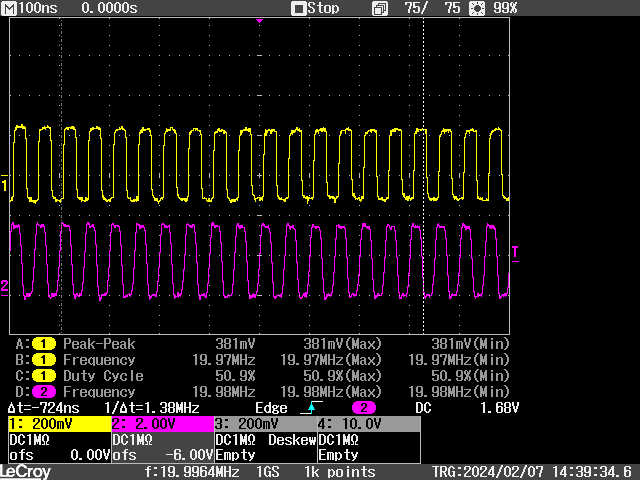
\includegraphics[scale=0.45]{./Mereni/MCLOCK_DIFF_PROBE.png}
	\caption{Průběh komunikačního hodinového signálu Timepix 2.} 
	\label{fig:MCLOCK_DIFF_PROBE}
\end{figure}

\section{Měření teploty Timepix2}
\label{teplota}
Pixelový detektor Timepix 2 umožňuje monitorovat vnitřní teplotu detektoru. Hodnota výsledné teploty detektoru je poté dle simulace teploty detektoru v závislosti na napěťové referenci popsána na obrázku \ref{fig:tpx2_temp}. Pro získání teploty detektoru je zapotřebí naměření dvou analogových hodnot z obrázku \ref{fig:tpx2_temp}, označovaných jako Vtemp a Vbg. Pro získání těchto analogových hodnot je nejprve zapotřebí nastavit, jaká hodnota analogového napětí bude na výstupu pinu Timepix 2 označovaného jako DACOUT. Výstup pinu DACOUT Timepix 2 je poté zpracován interním 12-bitovým AD převodníkem mikrokontroléru na základní desce \ref{zakladni deska}. Příklad výběru hodnoty na výstup DACOUT detektoru Timepix 2 a převod získané hodnoty na odpovídající teplotu lze vidět v zjednodušeném kódu \ref{kod_temp_tpx2}. Zpracovaná teplota je následně odeslána do programu TrackLab. Zobrazení teploty v programu TrackLab detektoru Timepix 2 lze najít na obrázku \ref{fig:Tracklab}.  
\begin{figure}[h!]
	\centering
	\captionsetup{justification=centering}
	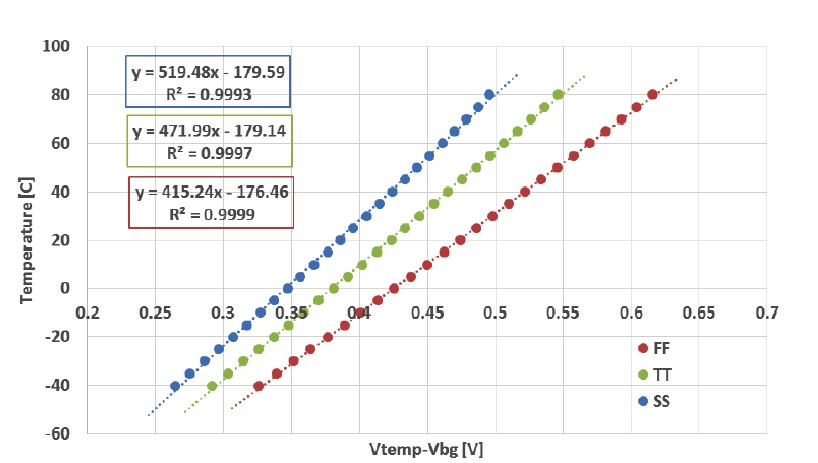
\includegraphics[scale=0.50]{tpx2_temp.jpg}
	\caption{Simulace teploty detektoru Timepix 2 v závislosti na hodnotě napěťové reference \cite{tpx2_manual}.} 
	\label{fig:tpx2_temp}
\end{figure}

\begin{lstlisting}[frame=single, language=C, caption={Výběr výstupu DACOUT detektoru Timepix2 a odečtení hodnoty detektoru.}, label=kod_temp_tpx2]
	// GET DAC : VBG_TEMP
	uint8_t set_dacoutsel[0] = VBG_TEMP; 
	float vtemp = 0;
	// set what type of DAC will be on DACOUT output								   
	if(tpx2_set_reg_8b(TPXA, SET_DACOUTSEL, set_dacoutsel) != TPX_OK) {    
		Error_Handler();
	}
	if(board_tpx2_get_dacout(TPXA, &vtemp) != BOARD_OK) {
		Error_Handler();
	}
	// Sim. -> TT. // Temp. into real value in ^C.
	float tpx2_temp = 471.99*(vtemp - vbg)/1000 - 179.14;					
\end{lstlisting}

\section{Digitální test Timepix 2} %popis prubehu a vysledku
Funkčnost komunikace s detektorem Timepix 2 byla, ověřena pomocí digitálních testů, jednotlivé testy budou popsány v následujících částech.
	\subsection{Vyčtení chip ID}
	Prvním digitálním testem, který byl implementován byl test, který vyčítá sériové výrobní číslo detektoru, označované jako CHIP ID, které je pro každý detektor Timepix 2 jedinečné a předem známé. Pro správné vyčtení CHIP ID detektoru je nejprve zapotřebí přivést napájecí napětí +2.5 V na pin VDD33, jak bylo popsáno v části \ref{Technicka specifikace}. Hodnota CHIP ID je poté uložena v 32-bitové registru Timepix 2. Vyčtením tohoto registru dostáváme 32 bitovou hodnotu, kterou pomocí známé transformace převedeme na skutečnou hodnotu CHIP ID, která odpovídá předem známému sériovému číslu detektoru Timepix 2. Program TrackLab, před každým připojením nového rozhraní vyčte sérové číslo připojeného detektoru. Výpis získaného CHIP ID v programu TrackLab lze vidět na obrázku \ref{fig:Tracklab}.

	\subsection{Vyčtení a zapsání pixelových matic}
	Pomocí výše uvedeného testu, vyčtení CHIP ID detektoru došlo k otestování vyčítaní základních registrů detektoru Timepix 2. Dalším digitálním testem je poté zápis a vyčtení všech digitálních čítačů, používajících se pro měření. Popis čítačů Timepix 2, lze najít v části \ref{Digitálni cast}.
	\par Zápis do digitálních čítačů slouží jen pro digitální testování, při samotném měření se tato funkce nevyužívá. S výjimkou nastavení konfigurační matice a matice lokálních prahových úrovní, které se využívají pro nastavení 10-bitového a 4-bitového čítače. Celkem při digitálním testu došlo k zápisu hodnot do všech dostupných čítačů Timepix 2 a následnému vyčtení. Celkem bylo zapsáno 5 testujících obrazů. Zapsané obrazy byly zvoleny dle tabulky \ref{tab:obraz}. Při digitálním testu tedy došlo k zápisu 327 680 B dat a jejich opětovnému vyčtení. Digitální test byl prováděn s frekvencí datových hodin 40 Mhz. Po každém digitálním testu bylo resetováno napájení detektoru Timepix 2 a digitální test byl proveden znovu. Při opakovaném digitálním testu, nebyly pozorovány problémy.
	\begin{table}[h!]
		\centering
		\begin{tabular}{ |P{3cm}|P{4cm}|  }
			\hline
			\multicolumn{2}{|c|}{Vybrané zapsané obrazce} \\
			\hline
			Test  & Obraz\\ \hline \hline 
			1 & 0xFF \\ \hline 	
			2 & 0x00 \\ \hline 		 
			3 & INC (0x00, 0x01, ..) \\ \hline
			4 & DEC (0xFF, 0xFE, ..)\\ \hline
			5 & 0xAA\\ \hline
		\end{tabular}
		\caption{Digitální test Timepix 2, zapsané hodnoty.}
		\label{tab:obraz}
	\end{table}
\section{Vyčítaní DAC převodníku Timepix 2}
	Dalším testem ověřujícím funkčnost navrženého vyčítacího rozhraní byl sken interních DAC Timepix 2. Test při kterém do 18 interních DAC kanálů detektoru Timepix 2 byla pro každý kanál zapsána digitální 8-bitová hodnota v rozsahu 0 až 255. Následně byl jednotlivě zvolen DAC kanál, který bude výstupem na pinu DACOUT detektoru Timepix 2. Tato výstupní, již analogová hodnota z výstupního pinu DACOUT byla převedena interním 12-bitovým AD převodníkem mikrokontroléru. Princip volby, které DAC bude na výstupu pinu DACOUT je analogický s popsaným kódem v části \ref{teplota}. DAC sken pro 18 interních DAC kanálů s výpisem do programu TrackLab můžete vidět na obrázku \ref{fig:dacscan}. 
	\begin{figure}[h!]
		\centering
		\captionsetup{justification=centering}
		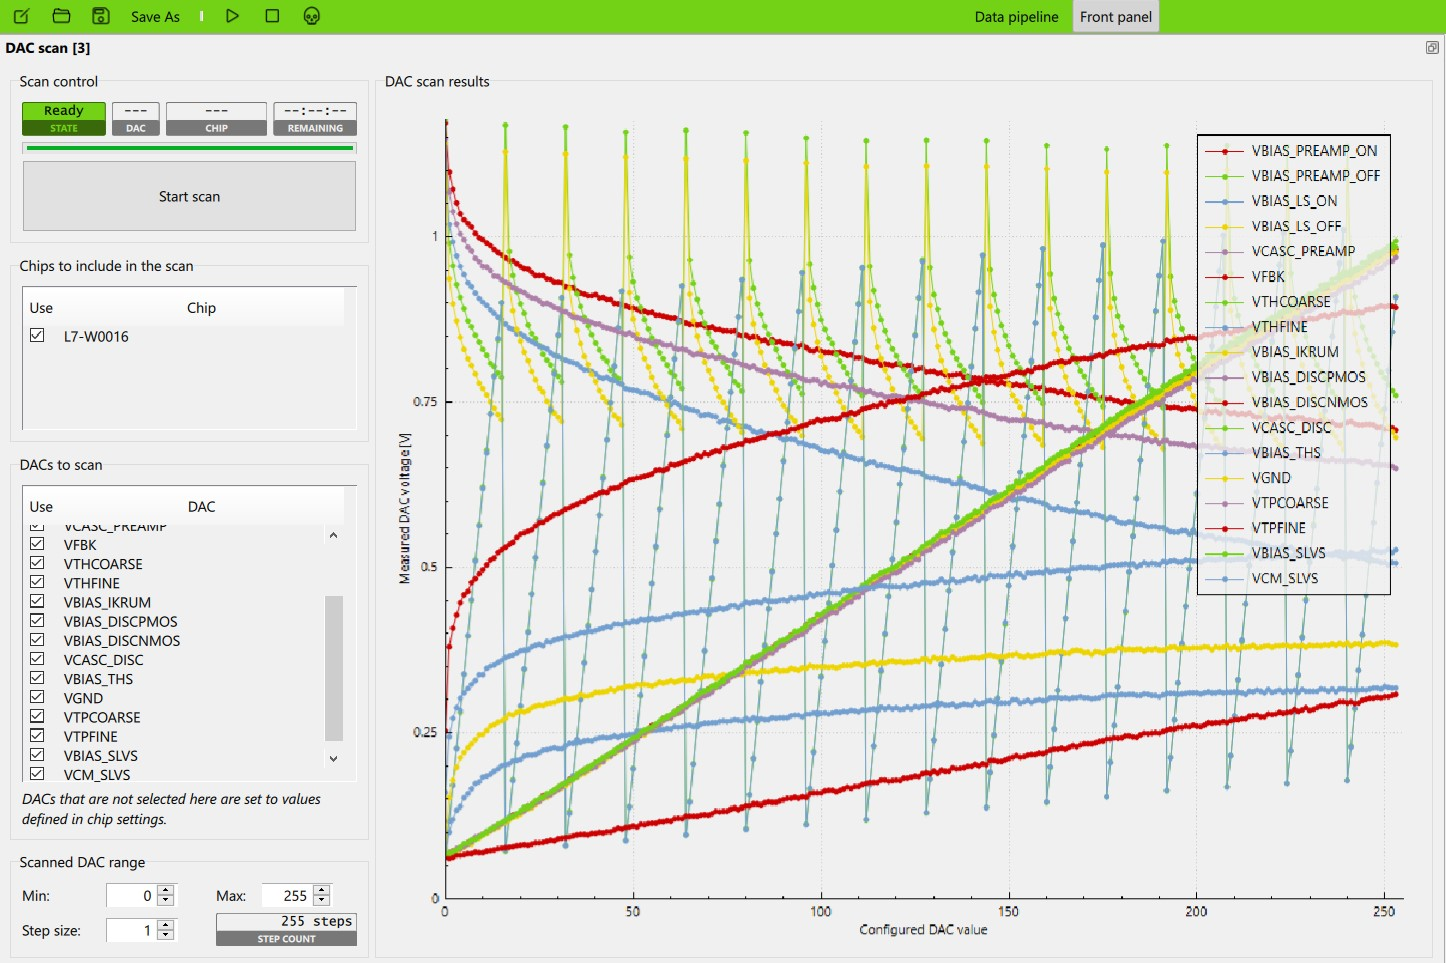
\includegraphics[scale=0.35]{tracklab_dac.jpg}
		\caption{Zobrazení vyčtených hodnot DAC převodníků Timepix 2 v celém rozsahu.} 
		\label{fig:dacscan}
	\end{figure}

\section{Ekvalizace Timepix 2}
	Komplexním testem testující spolehlivou funkčnost navrženého rozhraní byl proces ekvalizace detektoru Timepix 2 v programu TrackLab. Jak bylo popsáno v části \ref{analog}, každý z 256 x 256 pixelů matice obsahuje lokální DAC převodník pro nastavení lokální prahové úrovně detekovatelného signálu. Právě tato lokální úroveň detekovatelného signálu je optimalizačně nastavována z programu TrackLab. Další funkcionalita Timepix 2 čipu využívající se při ekvalizaci čipu je možnost maskování pixelů. Neboli pixel, který byl vybrán jako maskovací, vypíná daný pixel. Kombinací maskování pixelů a optimalizačního výběru lokálních prahových úrovní lze získat parametry potřebné pro nastavení detektoru Timepix 2, aby byl minimalizován šum detektoru. Prvním získaným parametrem je takzvaná matice lokálních prahových úrovní. Neboli matice 256 x 256 x 5 bitů nesoucí informaci, jakou 5-bitovou lokální úroveň nastavit pro daný pixel. Dalšími parametry jsou maskovací matice a hodnota globální prahové úrovně. Maskovací matice, jak již bylo popsáno nese informaci, jaký pixel z matice má být zamaskován, či odmaskován. Globální prahová úroveň je poté společná úroveň detekovatelného signálu pro celý detektor. Výsledek ekvalizace z programu TrackLab můžete vidět na obrázku \ref{fig:tracklab_eql}. Kdy globální prahová úroveň byla vypočítaná jako 2068 se směrodatnou odchylkou 5.97. Získaná globální prahová úroveň je poté převedena na digitální hodnotu pomocí známé transformace a následně zapsána do detektoru Timepix 2.
	\begin{figure}[h!]
		\centering
		\captionsetup{justification=centering}
		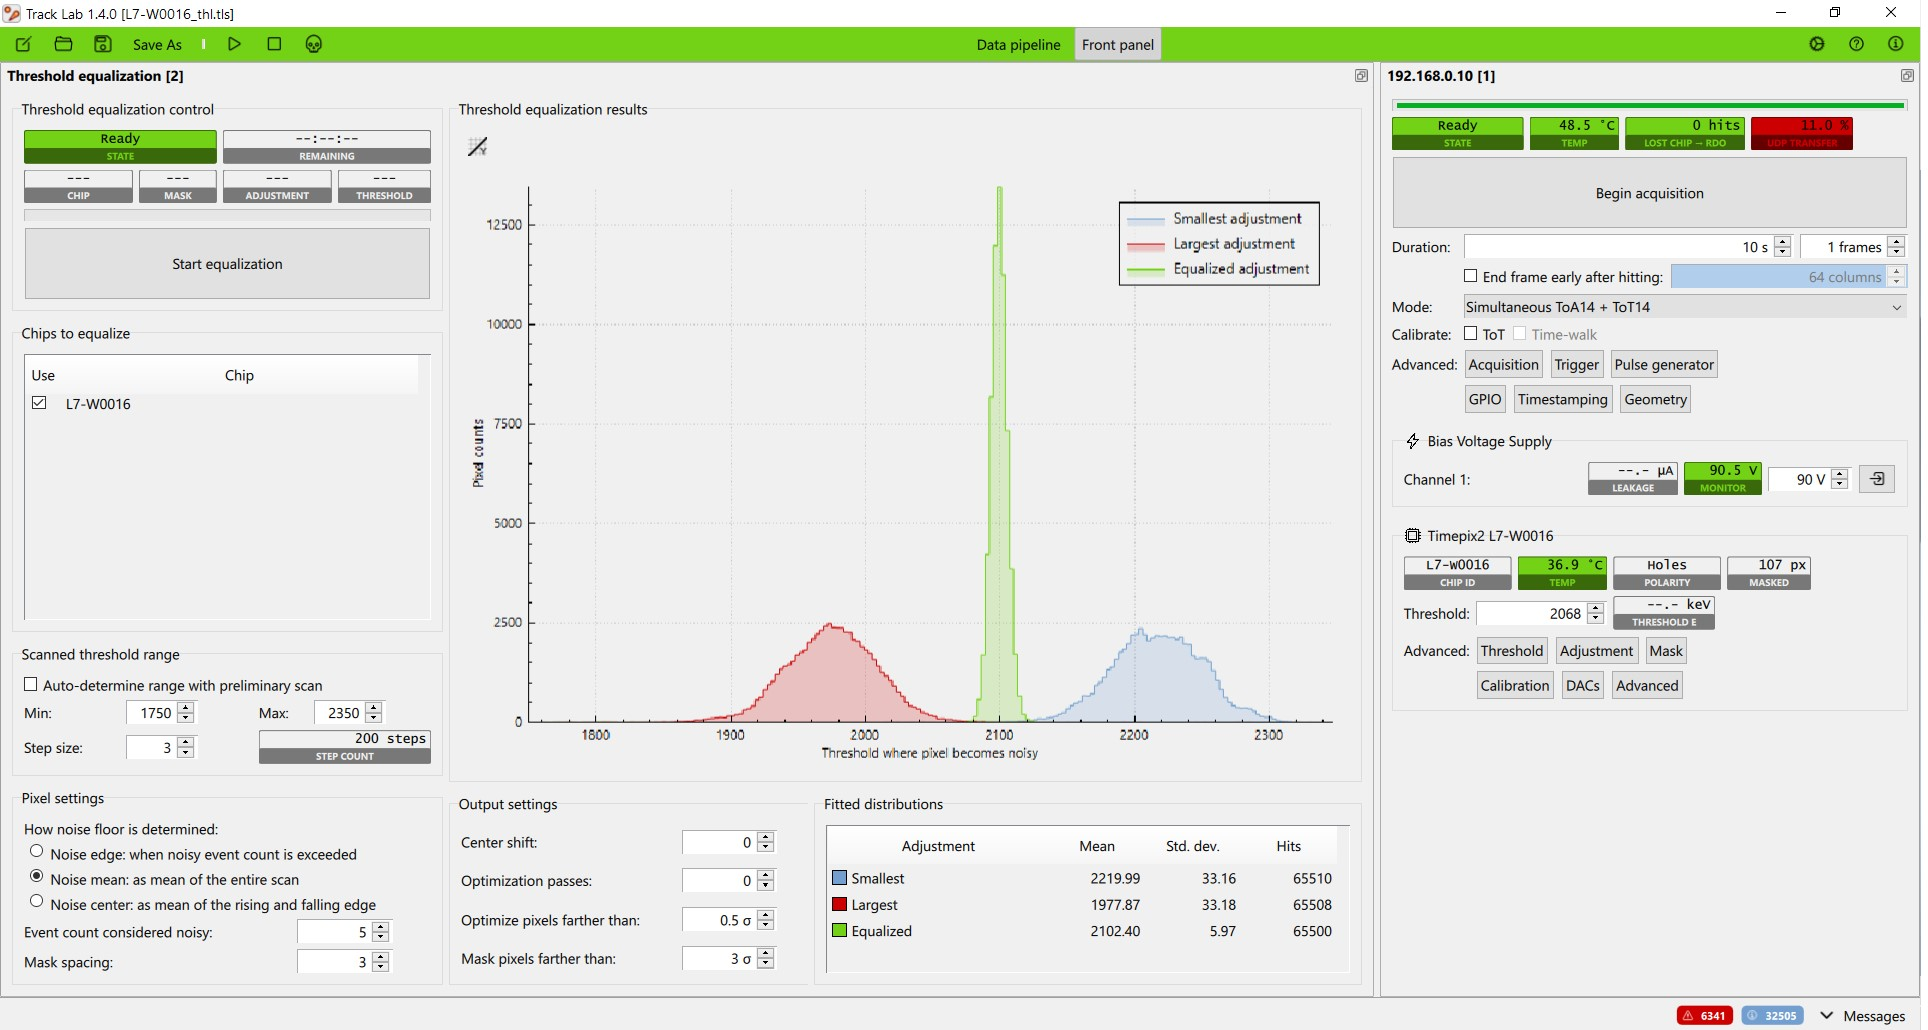
\includegraphics[scale=0.35]{tracklab_eql.jpg}
		\caption{Ekvalizace Timepix 2 čipu z programu TrackLab.} 
		\label{fig:tracklab_eql}
	\end{figure}

% TODO DOPOCITAT a vysledky
\section{Měření v laboratoři CERN}
	Posledním testem navrženého vyčítacího rozhraní bylo měření na urychlovači částic Proton Synchrotron (PS) \cite{PS} v laboratoři CERN \cite{CERN}. Parametry urychlených částic je možné najít v tabulce \ref{tab:castice}. Jednalo se o pozitivn9 nastavení urychlovače, tedy svazek byl zhruba z 80$\%$ tvořen protony a z 20$\%$ piony. 
		\begin{table}[h!]
		\centering
		\begin{tabular}{ |P{1.5cm}|P{2.5cm}|P{2.5cm}|P{3cm}|P{2.5cm}|  }
			\hline
			\multicolumn{5}{|c|}{Parametry urychlených částic} \\
			\hline
			Částice & Energie [GeV] & Počet částic [-] & Doba svazku [ms] & Frekvence [Hz]\\ \hline \hline 
			Hadrony & 10 & $10^6$ & 400 & 0.05 \\ \hline 	
		\end{tabular}
		\caption{Parametry urychlených částic, z urychlovače Proton Synchotron v CERNu}
		\label{tab:castice}
	\end{table}

\subsection{Umístění rozhraní}	
	Navržené vyčítací rozhraní bylo umístěno do vyúsťujícího svazku z uvedeného urychlovače PS. Přesněji do středu svazku byl umístěn detektor Timepix 2. Rozhraní bylo přimontováno na rotační a posuvný stůl, který je možné vidět na obrázku \ref{fig:setup_meas_beam}. Pozice zařízení byla možná měnit ve třech osách. Pomocí dvou posuvných os bylo zařízení přesně umístěno do středu svazku vyúsťujícího z urychlovače částic. Pomocí rotační osy byl pak volen úhel natočení vyčítacího rozhraní vůči svazku. Celé rozložení navrženého experimentu je možné vidět na obrázku \ref{fig:setup_meas_beam}. Pozice vyčítacího rozhraní vůči středu svazku je poté zobrazena na obrázku \ref{fig:setup_meas_beam_1}. Posledním nastavením experimentu bylo analogické z obrázků \ref{fig:setum_beam}, jedinou změnou pak bylo natočení celého rozhraní o 90$\deg$ vůči svazku.
	
\subsection{Nastavení měření}	
	Dle parametrů urychlených částic z uvedené tabulky \ref{tab:castice}, bylo měření s detektorem Timepix 2 následovné. Detektor byl nastaven do režimu s názvem: column trigger. V tomto režimu je možné monitorovat obsazení sloupců pixelové matice. Pokud toto obsazení překročí nastavenou hodnotu, je ukončeno měření a data jsou vyčtena z rozhraní do programu TrackLab. Druhou možností, kdy jsou data vyčtena z rozhraní je po uplynutí nastaveno měřícího času. Konkrétněji nastavení měřící doby bylo 2s a počet obsazených sloupců, při kterém dojde k odeslání dat byl optimalizován v závislosti na staveném úhlu rozhraní vůči svazku.
	
\subsection{Vyhodnocení měření}
	Na obrázcích \ref{fig:tracks} můžete vidět vybrané snímky pořízené detektorem, během měření. Lze na nich pozorovat závislostt závislost délky stopy interagující částice na velikosti nastaveného úhlu. S rostoucím úhlem natočení detektoru vůči svazku se snižuje počet detekovaných částic, vlivem nastaveného režimu column trigger. Pokud se detektor otočí o 90$\deg$ je možné detekovat větší množství částic, protože dopadající částice dopadají v ideálním případě rovnoběžně na sloupce detektoru.
	
	\par
	Při měření byla použita křemíková senzorová vrstva o tloušťce 500$\mu$m. Na tuto vrstvu bylo připojeno vysoké napětí o velikosti 110 V. Detekovatelné částice zanechají v senzorové vrstvě pouze část své energie. Vrstva není na tolik tlustá, aby interagující částice zanechaly veškerou energii právě v této vrstvě. Pokud ze získaných snímků vyfiltrujeme stopy částic, které jsou způsobeny pouze urychlenými částicemi dostaneme snímky obsahující pouze stopy od urychlených částic. Následně pro každou stopu částice spočítáme čas TOT \ref{item:modes}, tedy čas kdy signál v daném pixelu byl nad nastavenou detekovatelnou úrovní. Toto provedeme pro každou stopu částice individuálně a vyneseme do grafu. V grafu \ref{fig:0deg_graph}, pak můžete vidět spektrum zanechané energie v senzorové vrstvě pro úhel 0$\deg$ natočení vyčítacího rozhraní vůči dopadajícímu svazku. Jak je vidět, rozložení naměřených dat odpovídá Landau pravděpodobnostnímu rozdělení. %TODO Landaou rozdeleni?
	
	\begin{figure}[h!]
		\captionsetup{justification=centering}
		\begin{subfigure}{0.5\textwidth}
			\centering
			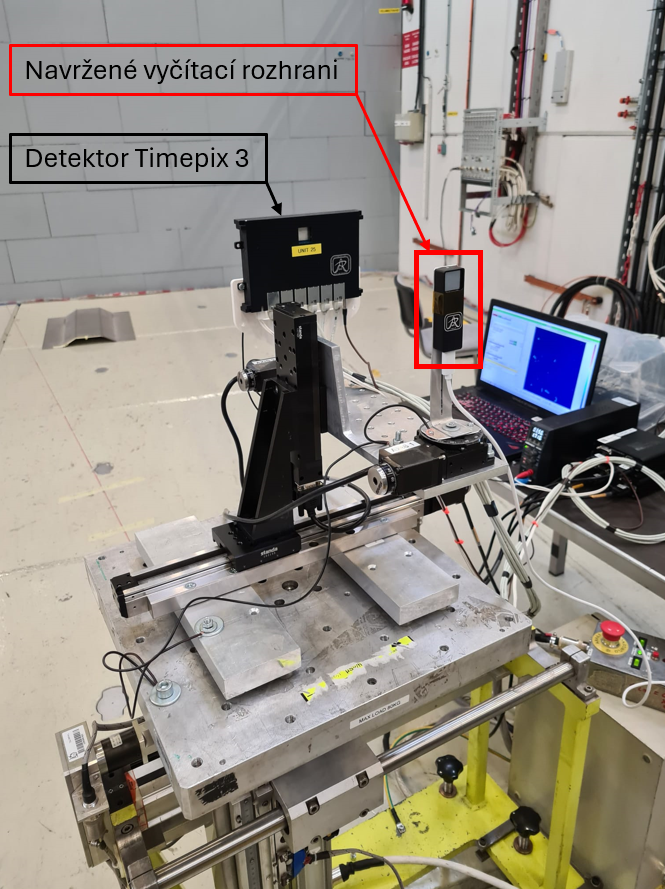
\includegraphics[scale=0.38]{setup_meas_beam.png}
			\caption{Pohled ze směru svazku na vyčítací rozhraní}
			\label{fig:setup_meas_beam}
		\end{subfigure}
		\begin{subfigure}{0.5\textwidth}
			\centering
			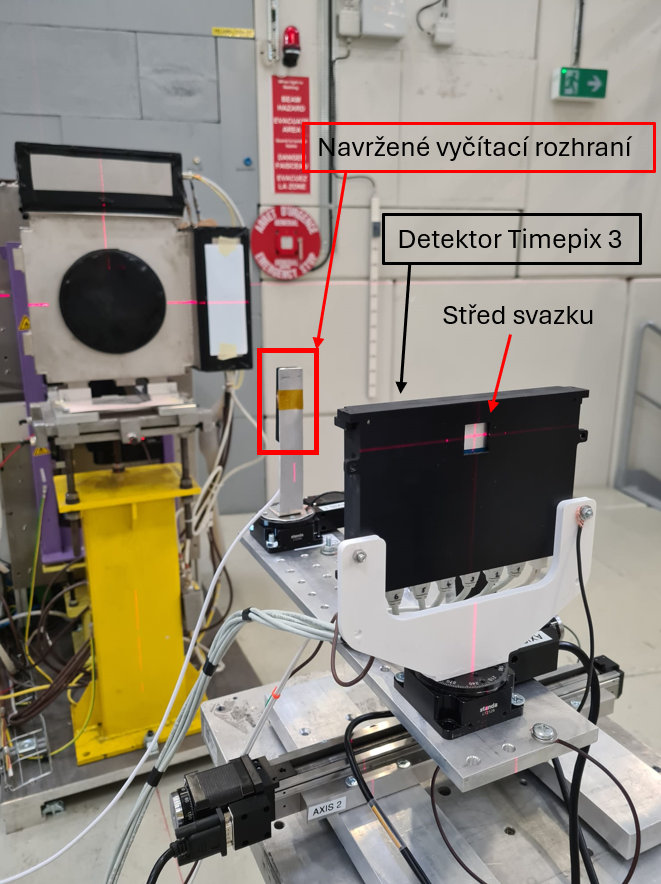
\includegraphics[scale = 0.38]{setup_meas_beam_1.png}
			\caption{Pozice vyčítacího zařízení vůči středu svazku}
			\label{fig:setup_meas_beam_1}
		\end{subfigure}
		\caption{Umístění detektorů vůči svazku z urychlovače částic}. %
		\label{fig:setum_beam}
	\end{figure}
	
	\begin{figure}[h!]
		\centering
		\captionsetup{justification=centering}
		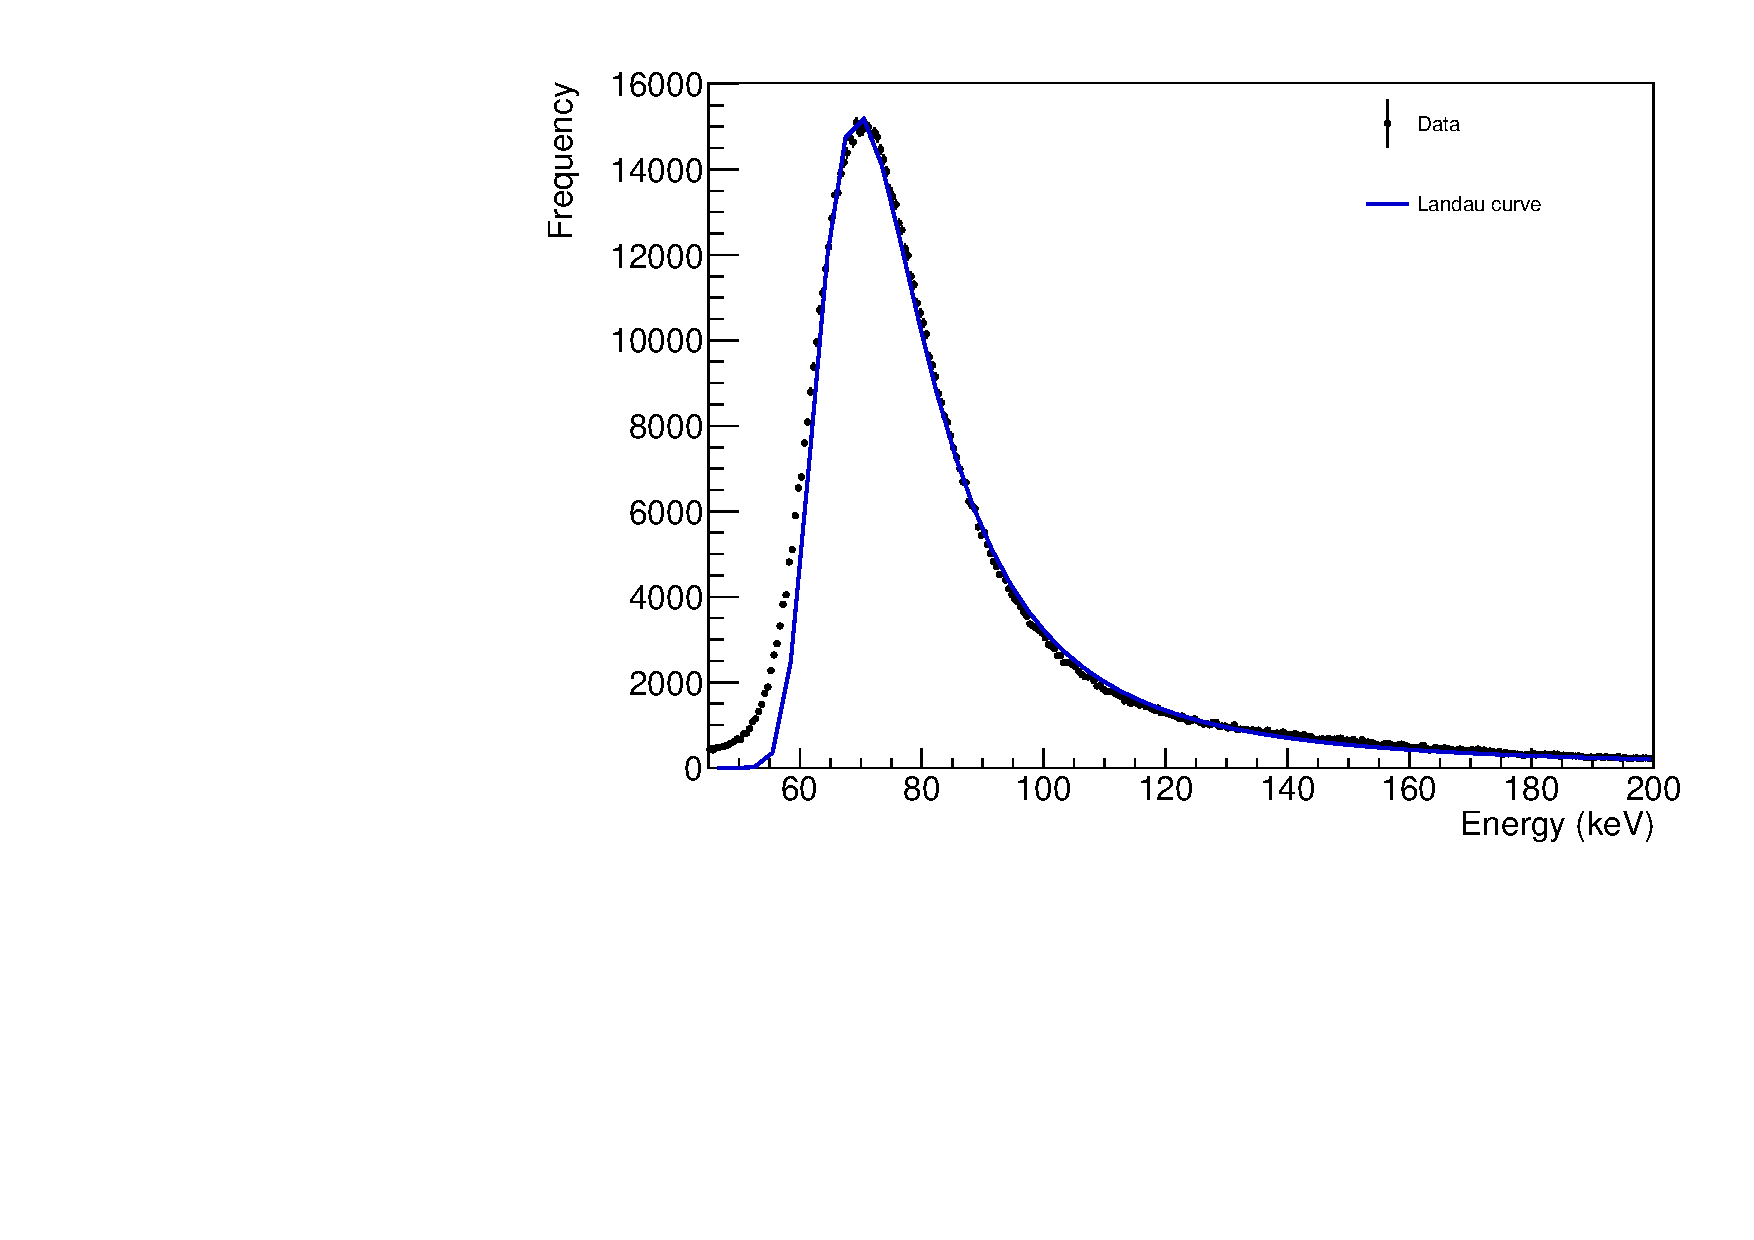
\includegraphics[scale=0.55]{0degrees_energy_spec_landau_model.pdf}
		\caption{Spektrum zanechané energie v senzoru pro pro úhel natočení 0$\deg$} 
		\label{fig:0deg_graph}
	\end{figure} 

	
	    \begin{figure*}
		\centering
		\begin{subfigure}[b]{0.475\textwidth}
			\centering
			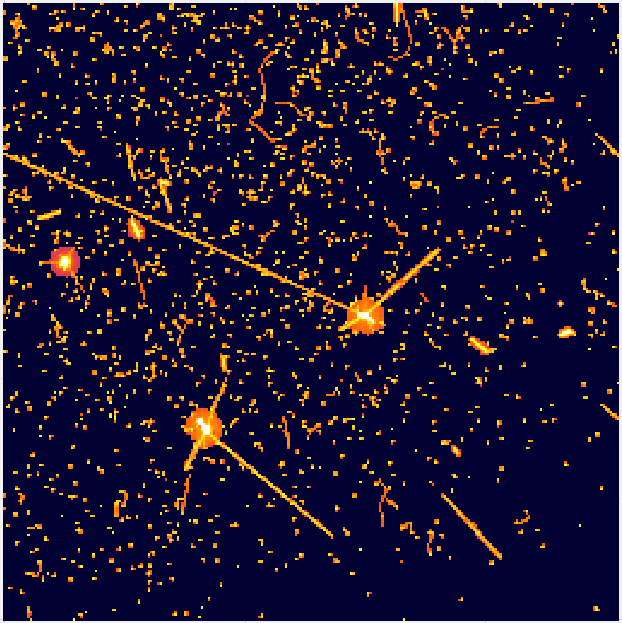
\includegraphics[width=\textwidth]{./beam/0deg/10GeV_hadrons_0deg_3.png}
			\caption{Úhel 0$^{\circ}$}
			\label{fig:0}
		\end{subfigure}
		\hfill
		\begin{subfigure}[b]{0.475\textwidth}  
			\centering 
			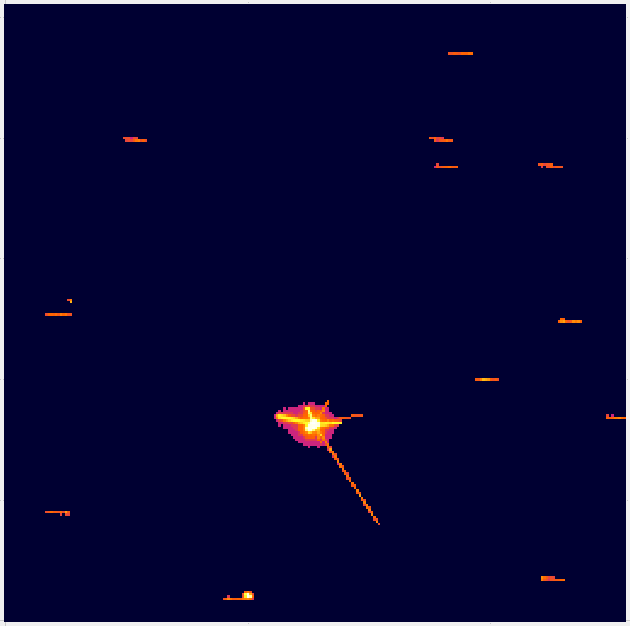
\includegraphics[width=\textwidth]{./beam/50deg/10GeV_hadrons_50deg_rep_99.png}
			\caption{Úhel 50$^{\circ}$}
			\label{fig:50}
		\end{subfigure}
		\vskip\baselineskip
		\begin{subfigure}[b]{0.475\textwidth}   
			\centering 
			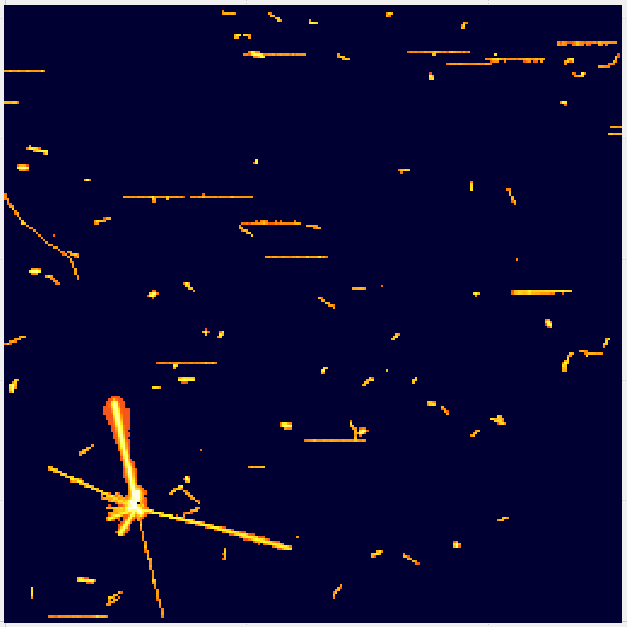
\includegraphics[width=\textwidth]{./beam/70deg/10GeV_hadrons_70deg_6_3}
			\caption{Úhel 70$^{\circ}$}
			\label{fig:70}
		\end{subfigure}
		\hfill
		\begin{subfigure}[b]{0.475\textwidth}   
			\centering 
			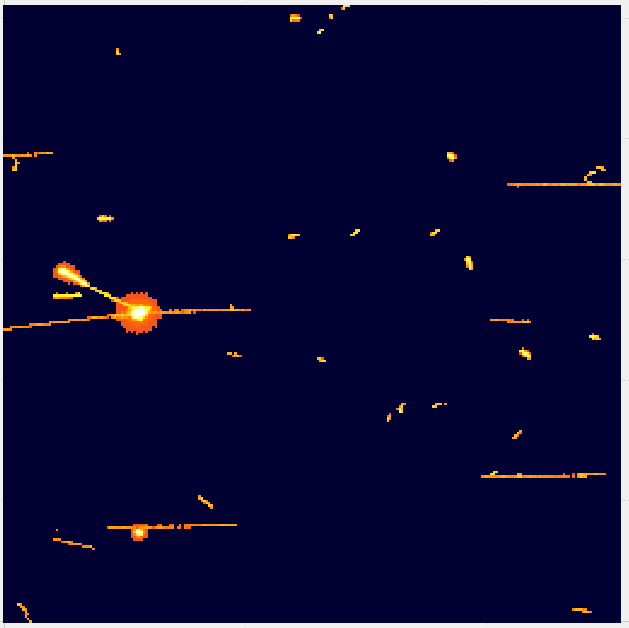
\includegraphics[width=\textwidth]{./beam/80deg/10GeV_hadrons_80deg_4_1}
			\caption{Úhel 80$^{\circ}$}
			\label{fig:80}
		\end{subfigure}
		\captionsetup{justification=centering}
		\caption[]
		{Snímky pořízené vyčítacím rozhraním, s různým úhlem natočením detektoru Timepix 2, vůči svazku.} 
		\label{fig:tracks}
	\end{figure*}

\section{Dosažené parametry}
Navržené vyčítací rozhraní bylo otestováno výše popsanými testy funkčnosti. Na základně těchto testů je možné stanovit parametry navrženého vyčítacího rozhraní viz tabulka \ref{tab:parametry}.

	\begin{table}[h!]
	\centering
	\begin{tabular}{ |P{7cm}|P{3cm}|P{2cm}|  }
		\hline
		\multicolumn{3}{|c|}{Parametry navrženého vyčítacího rozhraní} \\
		\hline
		Parametr & Hodnota &Jednotky\\ \hline \hline 
		Rozměry & 73.4 x 22 x 13.5 & [mm]\\ \hline 	
		Hmotnost & 35 & [g]	\\ \hline
		Spotřeba TPX2 ON & 1455 & [mW]\\ \hline
		Spotřeba TPX2 OFF & 825 & [mW]\\ \hline
		Rychlost vyčítaní dat z TPX2 & 40 & [Mbit/s]\\ \hline
		Max. rychlost vyčítaní dat z rozhraní & 480 & [Mbit/s]\\ \hline
	\end{tabular}
	\caption{Parametry navrženého vyčítacího rozhraní}
	\label{tab:parametry}
\end{table}

